%-------------------------------------------------------------------------------
% File: simulation.tex
%       Epidemic Broadcast project documentation.
%
% Author: Marco Pinna, Rambod Rahmani, Yuri Mazzuoli
%         Created on 05/12/2020
%-------------------------------------------------------------------------------

\chapter{Simulation}\label{simulation}
As we previusly described, we decided to consider a population of 100 users in two different scenarios:
\begin{itemize}
    \item \textbf{Small}: 10mx10m floorplan, with the transmission range going from 1m to 4.5m, with 0.5m steps, and
        the Bernullian base p going from 0.05 to 0.95 with 0.05 steps; 
    \item \textbf{Big}: 100mx100m floorplan, with the transmission range going from 1m to 19m, with 1m steps, and
        the Bernullian base p going from 0.1 to 0.9 with 0.1 steps; 
\end{itemize}
In order to acheive meaningfull results with a minumum accurancy of 90\%, we decide to repeat the same scenario with
the same parameters for 200 times, and than compute mean values from performance indexes, alogn with their confidence intervals.

\section{Big}\label{big}
\subsection{Coverage}
This plot show the coverage achived in function of P, for different values of R.
\begin{figure}[H]
    \begin{center}
        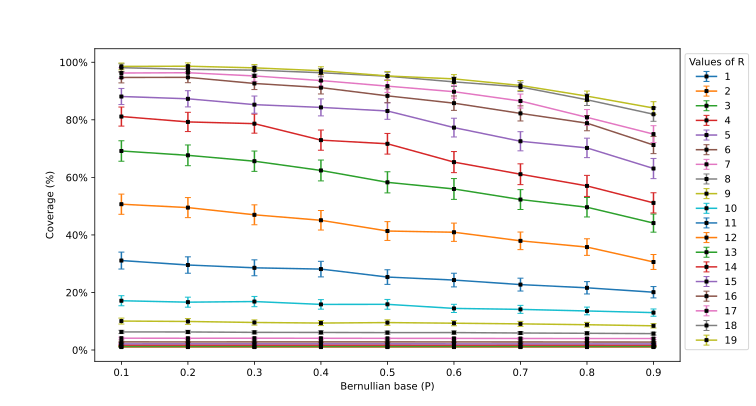
\includegraphics[scale=0.45]{img/Big_CovP.pdf}
        \caption{Big: Coverage vs P}
    \end{center}
    \vspace*{-1cm}
\end{figure}
As we can observe, the coverage we can reach is maximum when P is low; this was predictable by the fact that a low transmission
probability minimize the number of collisions, increasing the number of correct transmissions. 